%% Beginning of file 'sample631.tex'
%%
%% Modified 2021 March
%%
%% In particular, revtex v4.1 can be found at 
%% https://www.ctan.org/pkg/revtex4-1.

\documentclass[twocolumn,dvipsnames]{aastex631}
% twocolumn,linenumbers

\usepackage{xspace}
\usepackage{amsmath}
\usepackage{soul}
% \usepackage{titlesec} %comment out if we want 2 cols
\usepackage{lipsum, babel}
\usepackage[shortlabels]{enumitem}

\newcommand{\sectionbreak}{\clearpage}

% software
\newcommand{\lk}{\texttt{lightkurve}\xspace}
\newcommand{\unpopular}{\texttt{unpopular}\xspace}
\newcommand{\tesssip}{\texttt{TESS-sip}\xspace}

% telescopes
\newcommand{\galah}{{\small GALAH}\xspace}
\newcommand{\apogee}{{\small APOGEE}\xspace}
\newcommand{\galex}{{\small GALEX}\xspace}
\newcommand{\lamost}{{\small LAMOST}\xspace}
\newcommand{\kepler}{\textit{Kepler}\xspace}
\newcommand{\tess}{\textit{TESS}\xspace}
\newcommand{\gaia}{\textit{Gaia}\xspace}

% variales
\newcommand{\solmass}{M$_\odot$\xspace}
\newcommand{\solrad}{R$_\odot$\xspace}
\newcommand{\app}{$\sim$}
\newcommand{\logg}{$\log g$\xspace}
\newcommand{\teff}{T$_\textrm{eff}$\xspace}
\newcommand{\feh}{[Fe/H]\xspace}
\newcommand{\mgfe}{[Mg/Fe]\xspace}
\newcommand{\bafe}{[Ba/Fe]\xspace}
\newcommand{\ali}{$A\textrm{(Li)}$\xspace}
\newcommand{\dnu}{$\Delta \nu$\xspace}
\newcommand{\numax}{$\nu_{\text{max}}$\xspace}
\newcommand{\muhz}{$\mu \text{Hz}$\xspace}
\newcommand{\halpha}{H-$\alpha$\xspace}
\newcommand{\vsini}{$v\sin i$\xspace}
\newcommand{\cc}{C$^{12}$/C$^{13}$\xspace}
\newcommand{\vbr}{$v_\textrm{broad}$\xspace}
\newcommand{\vmac}{$v_\textrm{macro}$\xspace}
\newcommand{\kms}{km s$^{-1}$\xspace}
\newcommand{\tc}{$T_c$\xspace}
\newcommand{\ang}{$\textrm{\AA}$\xspace}
\newcommand{\chisq}{$\chi^2$\xspace}

% repetitive words
\newcommand{\li}{lithium\xspace}
\newcommand{\lirich}{Li-rich\xspace}
\newcommand{\lin}{Li-normal\xspace}
\newcommand{\fthree}{\texttt{f3}}
\newcommand{\total}{1122\xspace}
\newcommand{\rotp}{rotation period\xspace}
\newcommand{\dg}{doppelg\"anger\xspace}
\newcommand{\dgs}{doppelg\"angers\xspace}
\newcommand{\plen}{planetary engulfment\xspace}
\newcommand{\seismo}{asteroseismology\xspace}
\newcommand{\ber}{beryllium\xspace}
\newcommand{\cond}{condensation temperature\xspace}
\newcommand{\pysyd}{\texttt{pySYD}\xspace}

\definecolor{forestgreen}{rgb}{0.13, 0.55, 0.13}
% 
\newcommand{\ask}[1]{\textbf{\textcolor{orange}{Ask: #1}}}
\newcommand{\done}[1]{\textbf{\textcolor{cyan}{#1}}}
\newcommand{\todo}[1]{\textbf{\textcolor{purple}{#1}}}
\newcommand{\gully}[1]{\textbf{\textcolor{forestgreen}{#1}}}
\newcommand{\ben}[1]{\textbf{\textcolor{blue}{#1}}}

%% Reintroduced the \received and \accepted commands from AASTeX v5.2
% \received{March 1, 2021}
% \revised{April 1, 2021}
% \accepted{\today}

%% Command to document which AAS Journal the manuscript was submitted to.
%% Adds "Submitted to " the argument.
%\submitjournal{PSJ}

\shorttitle{Brownian Rotation}
\shortauthors{Montet and/or Gully-Santiago}

%% \watermark{text}
%% \setwatermarkfontsize{dimension}
\graphicspath{{./}{figures/}}

\begin{document}

\title{Ben Brown's models are right, or maybe not, let's find out together}

\correspondingauthor{One of Us}
\email{email@email.edu}


\author[0000-0001-7516-8308]{Benjamin T. Montet}
\affiliation{School of Physics, University of New South Wales, Kensington, New South Wales, Australia}
\affiliation{UNSW Data Science Hub, University of New South Wales, Sydney, NSW 2052, Australia}


\author{Michael Gully-Santiago}
\affiliation{UT Austin}


\begin{abstract}
\todo{This is an abstract}

\end{abstract}

%% https://astrothesaurus.org
\keywords{Stars: abundances --- stars: activity --- stars: evolution --- stars: rotation --- stars: AGB and post-AGB}


\section{Introduction} \label{sec:intro}

M dwarf magnetic fields are poorly understood. 

Lots of theories out there of what might happen in the photometry.

One of these is Brown et al. 2020, who have models with hemispheric oscillations over $\sim$ 15 rotation periods

This should be detectable in long-term photometry, such as the Kepler FFIs

How can we characterise the variability on long timescales of fully convective objects?

\section{A little bit of theory}

Our metric is the amplitude of the short-term variability of a star's brightness, inferred as largely due to starspots, compared to the brightness in the \kepler\ bandpass overall, as inferred through \fthree\ photometry.

\subsection{What does this look like in activity cycles}

We would see something that goes up or down in time linearly, whether the star is spot or facula dominated. This is consistent with \citet{Montet17} and can be used to infer the relative importance of starspots and faculae in the overall brightness of individual stars from the Earth's viewing angle.

\subsection{What does this look like for Ben Brown's models?}

Well that's complicated by viewing angle which we don't understand. For stars that are equator-on (and have no long-term changes in the activity level, only a swap in active hemisphere), that should mean both the overall flux and short-term activity are constant. As the star becomes more pole-on, these two effects deviate: the overall short-term variability level decays as starspots remain visible and at similar levels of limb darkening over their entire rotation. The overall flux becomes more variable though, as the total spot coverage visible to an observer changes dramatically from the active hemisphere being visible towards Earth to the opposite case. 

\subsection{How do we test this?}

We don't know the inclination angles and this makes things hard. But we can use a control sample and large enough samples so that the unknown inclinations wash out over a population, and we can dive deep on individual systems to understand their specifics. 


\section{Data Processing}

Okay so the data are actually sub-optimal for this in some ways.

We want to explore the slower rotators. But for these, PDC warps the signal so that we don't see long-term signals in all quarters, and the ones we do, we're skeptical that the amplitude hasn't been modulated by the pipeline. We know this is the case at least sometimes!

So SAP is useful, but it has all sorts of long-term signals in it which are instrumental in nature. Those will stuff up our interpretation if we don't correctly account for them.

What do? Something like Christina's TESS-SIP is the way forward here, we can apply it to the SAP data and do a good job separating the instrumental and astrophysical signals. Better yet, when we do that, we have an additional piece of information in that we can anchor the flux to the \fthree\ flux at each month, which will help us model the long-term behavior. We know what is going on in intermediate timescales which helps us calibrate those short timescales.

lightkurve is a good bet here, because we can use the CBVCorrector class to get the CBVs, and add in extra terms to the design matrix on top of that easily. What are the necessary additional terms to add in? We need something that looks like the stellar variability via a periodic signal, the CBVs, and something that anchors the data at the times of the \fthree\ photometry. 


\section{Sample Selection}

The \citet{Brown21} model is based in fully-convective M dwarfs. We use the gaia-kepler.fun one-to-one catalog, which crossmatches Gaia DR3 against the Kepler DR25 catalog of all stellar targets with long-cadence observations from \kepler. We select all targets in this catalog with Gaia temperatures less than 3400 K and \logg $> 4.0$, to select M dwarfs near and below the fully convective boundary. As a control sample, we also select a sample of earlier M dwarfs, with $3400 < T < 3700$ and the same gravity constraint.


\section{Notes on Project Status}

Reminders to future us where we are and what specifically we're excited about:

\begin{itemize}

\item{We can test the Ben Brown theory of what's going on with these stars}
\item{We have a model using Brett Morris' starry of what activity variations should look like under the
standard model of spot evolution vs hemispheric magnetic reversal. They are different!
Specifically, there is a gap at moderate fluxes/low spot amplitudes that we don't expect to fill in with Brown's model. Can we see this in the data?}
\item{To do this we're going to look at the amplitude of variability on short timescales (e.g. inside a quarter) compared to the FFI flux, which we expect to be more or less a trend line under the standard model but follow a curve with a shoulder under the Brown model}
\item{To do this we need better measurements of rotation on long timescales. We're overfitting this right now, not as badly as PDC does, but still at some level. We have some ideas how do to this better, which will leverage the design matrix ecosystem}
\item{As a control sample of edge-on stars, we can look at the planet hosting stars, which should on average have high inclinations}
\item{Can we do this with MEarth too? Control sample being stars with known Rsini from rotation period + spectrum. Gaia RVS spectra good enough?!}

\end{itemize}

\begin{figure}
    \centering
    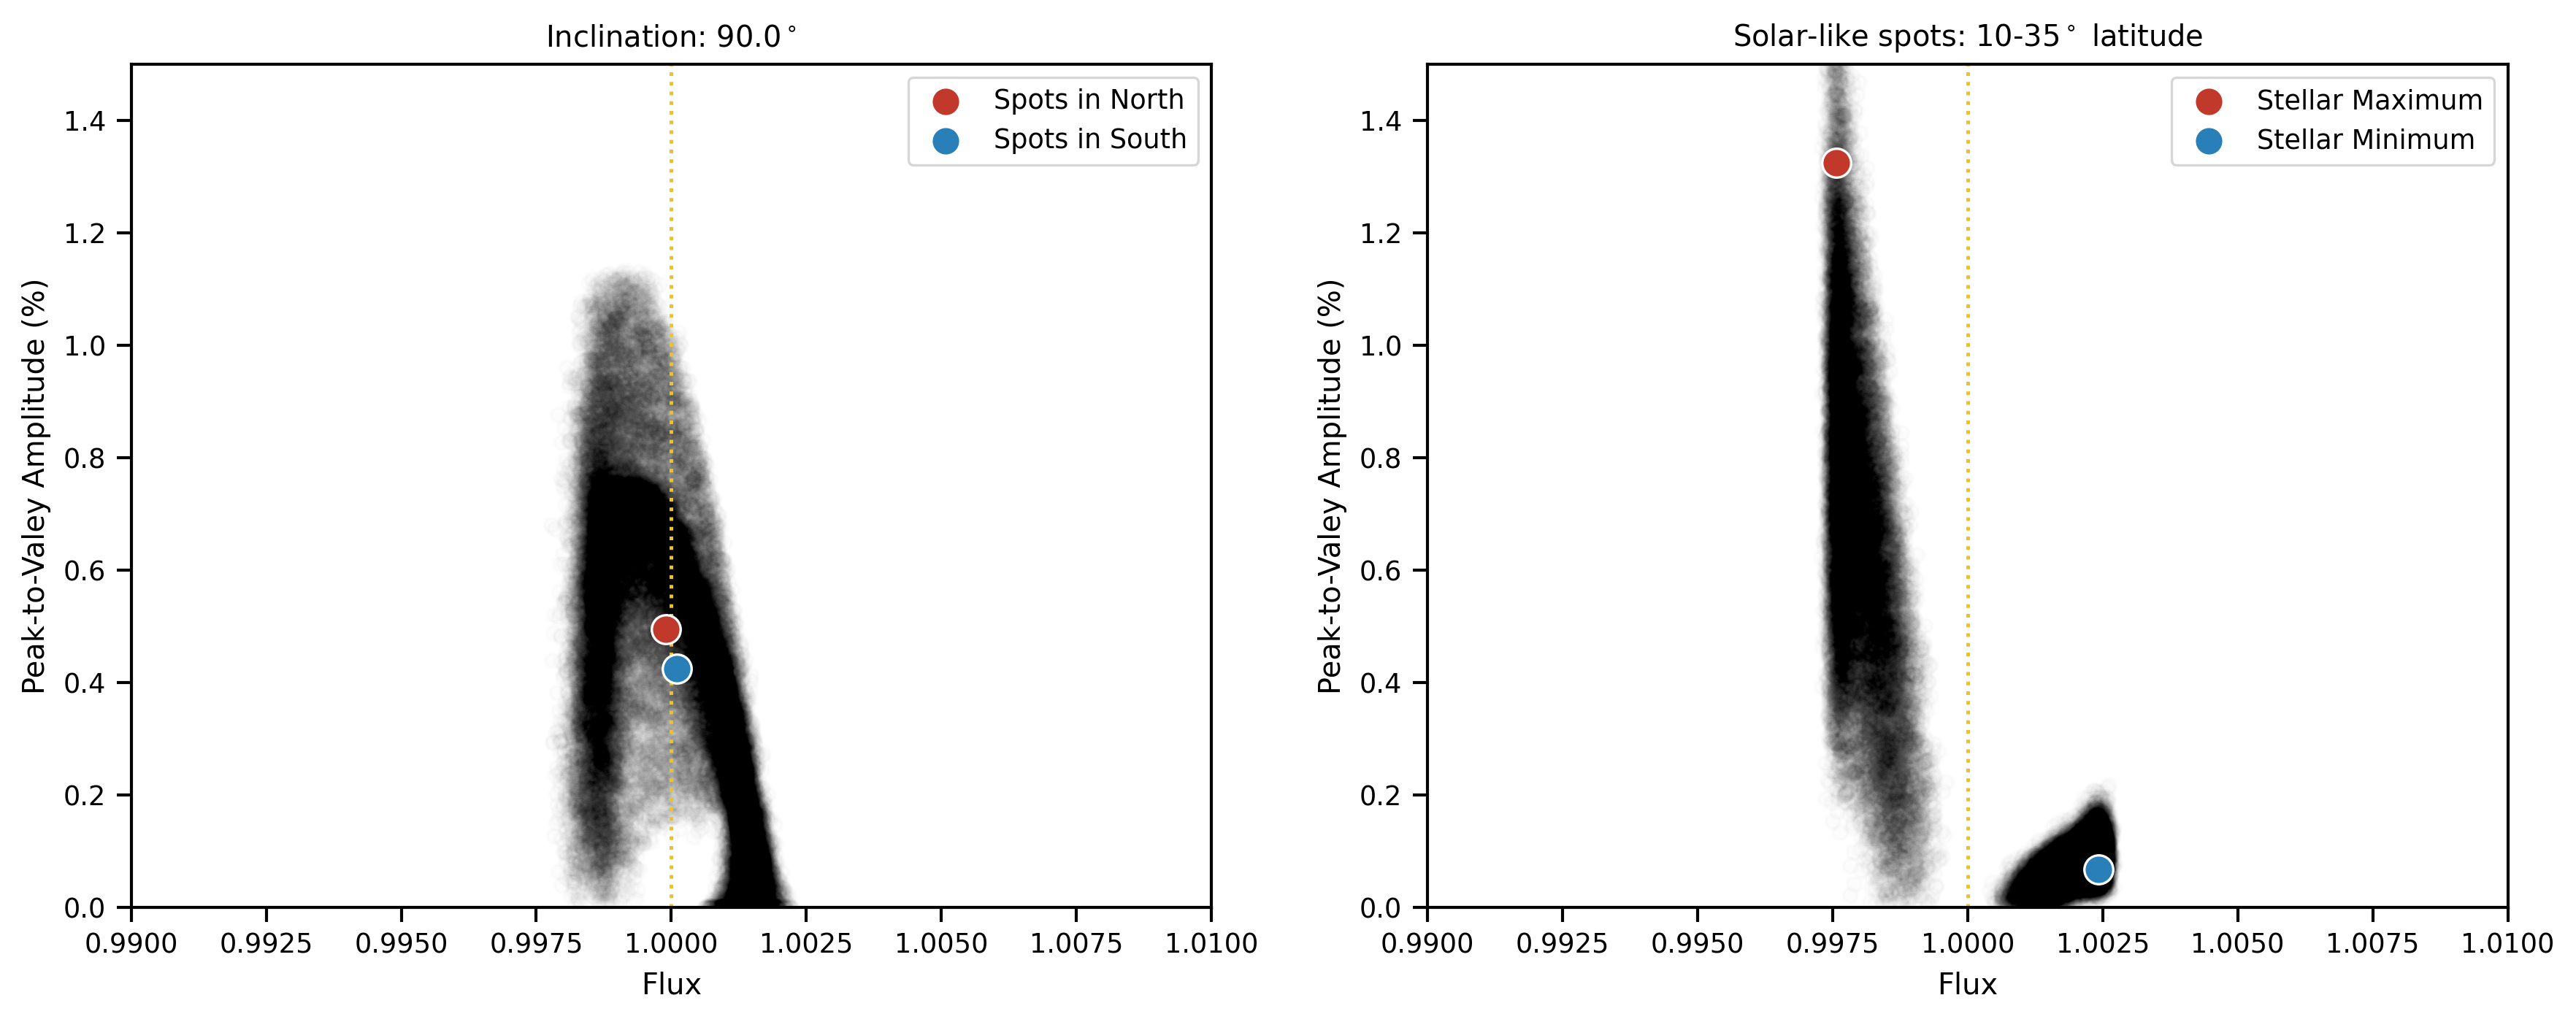
\includegraphics{figures/fleck_solar_like.png}
    \caption{Difference between the Brown model (left) and standard model, demonstrating the change in observed short-term and long-term variability between the most active and least active states.}
    \label{fig:fleck}
\end{figure}


\bibliography{references}{}
\bibliographystyle{aasjournal}


\end{document}

% End of file `sample631.tex'.
